\documentclass[cn,10pt,math=newtx,citestyle=gb7714-2015,bibstyle=gb7714-2015]{elegantbook}

\title{PerceptionX 面试官题库}

\author{Cheng Wang}
\date{Sep 14, 2021}
\version{0.1}

\extrainfo{Perception and beyond for autonomous driving -- PerceptionX}

\setcounter{tocdepth}{3}

% \logo{logo-blue.png}
\cover{cover.jpg}

% 本文档命令
\usepackage{array}
\usepackage{graphicx}
\usepackage{subfigure}

\newcommand{\ccr}[1]{\makecell{{\color{#1}\rule{1cm}{1cm}}}}

\definecolor{customcolor}{RGB}{32,178,170}
\colorlet{coverlinecolor}{customcolor}

\begin{document}

\maketitle
\frontmatter

\tableofcontents

\mainmatter

\chapter{编程与计算机基础}

\section{C \& C++}

\begin{introduction}
\item Array \& Pointer
\item Memory Models and Namespaces
\item Objects and Classes
\item Input, Output, and Files
\item Design Patterns
\item Multi-threading \& Multi-processing
\end{introduction}

适用于 \textbf{以 C 和 C++ 为主要编程语言、工程开发岗}  的候选人。

\subsection{Array \& Pointer}
%\problemset
\textbf{Q1.} \textit{申明一个 char 的数组,并且初始化为字符串 ``cheeseburger''。}

A1. 参考答案:
\begin{lstlisting} [language=c++]
char lunch[13] = "cheeseburger"; // 预留空间
char lunch[] = "cheeseburger"; // 或由编译器自行分配
\end{lstlisting}


\textbf{Q2.} \textit{C++ 中连续 delete 两次指针会出现什么问题,如何彻底解决连续两次 delete 的问题?}

A2. delete 只负责将内存标记为可用,不负责将指针置为 NULL。如果这部分内存尚未被复用,则会显示警告;如果已被系统或者其他程序复用,可能导致崩溃。

建议使用\textbf{智能指针}。\\


\textbf{Q3.} \textit{数组、vector、array 的访问是否可能越界?这三种类型的对象是否可以直接赋值拷贝?如果可以的话,是深拷贝还是浅拷贝?}

A3. 使用中括号访问元素时,这三种类型都可能出现越界。但 vector 和 array 提供了 at() 方法,使用 at() 时,将在\textbf{运行期间捕获非法索引}。

数组不能,需要逐元素复制;在保证 size 相同的情况下,array 和 vector 可以,为深拷贝。\\


\textbf{Q4.} \textit{简述 vector 是怎么做扩容的}

A4. 被动扩容:如果 vector 已满,在新增数据的时候,将分配一块更大的内存,首先将原来的数据复制过来,然后释放之前的内存,再插入新增的元素.

主动扩容:使用 reserve(int new\_size) 或者 resize(int new\_size,/*int init\_value*/) 函数导致的扩容。会改变 capacity() 的返回值,不改变 size() 的返回值。\\


\textbf{Q5.} \textit{C++ 中 map 是有序的吗?低层是通过什么实现的?C++ 中存在无序的字典吗?}

A5. 是。map 内部是红黑树,在插入元素时会自动排序。无序容器 unordered\_map 内部是散列表,通过哈希而不是排序来快速操作元素,使得效率更高。当不需要排序时选择 unordered\_map 的效率更高。\\


\textbf{Q6.} \textit{指针与引用的区别}

A6.指针是本身存储的所指向的对象的地址,而引用只是引用对象的别名。通过 sizeof 可以获取指针的存储空间的大小,而 sizeof 引用的话获取的引用对象的存储空间的大小。指针在初始化可为空,指针指向的对象可以改变,而引用则不能为空,必须和引用对象绑定,而且之后不能改变。\\


\subsection{Memory Models and Namespaces}

\textbf{Q1.} \textit{查看下列代码,分别针对变量 v\_1, v\_2, v\_3, v\_4 回答:a). 是否整个程序执行期间都存在;b). 能在 funct2 中使用吗?c). 能在程序的其他文件中使用吗?}

A1. 参考答案:

\begin{itemize}
  \item v\_1, v\_2, v\_3 在整个程序执行期间都存在,因为他们是静态持续变量。v\_4 只有在 funct1 执行时才存在;
  \item 只有 v\_1, v\_2 可以在 funct2 中使用;
  \item 只有 v\_1可以在程序的其他文件中使用\\
\end{itemize}

\begin{lstlisting} [language=c++]
int v_1 = 1000;
static int v_2 = 50;

int main()
{
...
}

void funct1(int n)
{
    static int v_3 = 0;
    int v_4 = 0;
...
}
void funct2(int q)
{
...
}
\end{lstlisting}


\textbf{Q2.} \textit{查看下列代码,回答关于声明空间的问题}

A2. 代码和参考答案:
\begin{lstlisting} [language=c++]
namespace sensetime {
    double user_id;
    struct attribute {...};
}

char user_id;

int main()
{
    using sensetime::user_id; // 该语句做了什么
    int user_id;
    cin >> user_id; // 此处键盘输入赋值给了哪个 user_id,为什么
    cin >> ::user_id; // 此处键盘输入赋值给了哪个 user_id,为什么
    cin >> sensetime::user_id; // 此处键盘输入赋值给了哪个 user_id,为什么
}
\end{lstlisting}

\subsection{Objects and Classes}

\textbf{Q1.} \textit{公有继承、受保护继承、私有继承的区别}

A1. 公有继承时,派生类对象可以访问基类中的公有成员,派生类的成员函数可以访问基类中的公有和受保护成员;私有继承时,基类的成员只能被直接派生类的成员访问,无法再往下继承;受保护继承时,基类的成员也只被直接派生类的成员访问,无法再往下继承。\\


\textbf{Q2.} \textit{在一个类 (例如 class A) 的成员函数中,return this 和 return *this 有什么区别?}

A2. return this 代表返回当前对象的地址 (指向当前对象的指针)。return *this 时,若返回值为 A,则返回当前对象的拷贝,若返回值为 A\&,则返回当前对象。\\


\textbf{Q3.} \textit{构造函数能不能是虚函数,为什么?}

A3. 不能。原因一:虚函数对应一个 vtable,vtable 存储在对象的内存空间。而对象还没有实例化时,是没有内存空间的。原因二:虚函数的作用在于通过父类的指针或者引用来调用它的时候可以变成调用子类的那个成员函数。而构造函数是在创建对象时自己主动调用的,不可能通过父类的指针或者引用去调用。因此,构造函数不能是虚函数。\\


\textbf{Q4.} \textit{C++ 中左值和右值的区别。左值和右值之间能互相转换吗?函数的返回值可以是左值吗?能否对右值添加引用?}

A4. 左值指既能够出现在等号左边,也能出现在等号右边的变量。左值是可寻址的变量,有持久性。

右值则是只能出现在等号右边的变量。右值一般是不可寻址的常量,或在表达式求值过程中创建的无名临时对象,短暂性的。

左值可以转换成右值,右值不能转换成左值。

函数的返回值可以是左值。例如返回一个变量的引用。

虽然 C++98/03 标准不支持为右值建立非常量左值引用,但允许使用常量左值引用操作右值。也就是说,常量左值引用既可以操作左值,也可以操作右值。C++11 标准新引入了另一种引用方式,称为右值引用,用 "\&\&" 表示。需要注意的,和声明左值引用一样,右值引用也必须立即进行初始化操作,且只能使用右值进行初始化。


\subsection{Input, Output, and Files}

\textbf{Q1.} \textit{解释 C++ 中流和缓冲区的概念}

A1. C++ 程序把输入和输出看作字节流。输入时,

\subsection{Design Patterns}

\textbf{Q1.} \textit{什么是工厂模式,适用于什么情况。}

A1. 工厂模式即定义一个用于创建对象的接口,让子类决定实例化哪一个类。工厂方法使得一个类的实例化延迟到其子类。\\

工厂方法的优点
\begin{itemize}
  \item 良好的封装性,代码结构清晰;
  \item 扩展性优秀。在增加产品类的情况下,只要适当的修改具体的工厂类或者扩展一个工厂类,就可以拥抱变化;
  \item 工厂模式是典型的解耦框架,高层模块只需要知道产品的抽象类,不需要关心其它的实现\\
\end{itemize}


\textbf{Q2.} \textit{什么是单例模式,适用于什么情况。}

A2. 一般情况下,我们建立的一些类是属于工具性质的,基本不用存储太多跟自身有关的数据,这种时候,每次都去 new 一个对象,既增加了开销,也使得代码更加臃肿。其实,我们只需要一个实例对象就可以了。若采用全局或静态变量的方式,会影响封装性,难以保证别的代码不会对全局变量造成影响。因此,我们将默认的构造函数声明为私有的,这样就不会被外部所 new 了,甚至可以将析构函数也声明为私有的,这样就只有自己能删除自己了。\\


单例模式的优点:
\begin{itemize}
  \item 单例模式只能有一个实例,减少了内存开支,特别是一个对象需要频繁的创建、销毁的类,只生产一个实例,也减少了系统的开销,当一个对象的产生需要比较多的资源的时候,如配置资源等产生其它依赖的对象时候,则可以通过这种设计模式在应用启动的时候就产生这个对象,然后用于驻留在内存中,可以直接取来使用;
  \item 避免对资源的多重占用;
  \item 在系统设置全局的访问点,优化和共享资源的方法\\
\end{itemize}


单例模式的缺点
\begin{itemize}
  \item 单例模式一般是没有接口的,如果想要扩展,除了修改代码基本没有其他方式,因为接口对单例模式是没有意义的,单例模式会自定实例化;
  \item 单例模式对测试不利,在并行开发环境中,如果单例模式没有完成,是不能进行测试的\\
\end{itemize}


使用场景:如果在系统中,要求一个类有且仅有一个对象,如果出现多个对象就会出现『不良反应』这种情况下就可以采用单例模式。如:

\begin{itemize}
  \item 生成唯一序列号的环境;
  \item 在整个项目中需要一个共享访问点或者共享数据;
  \item 创建一个对象需要消耗的资源过多,如访问 IO 和数据库等资源;
  \item 需要定义大量的静态常量和静态方法的环境
\end{itemize}


\subsection{Multi-threading \& Multi-processing}

\newpage


\section{Python}

\begin{introduction}
\item Function
\item Variable
\item Class \& Module
\item Input, Output, and Files
\item Multi-threading \& Multi-processing
\end{introduction}

适用于 \textbf{以 Python 为主要编程语言、算法研究岗、数据分析岗}  的候选人

\subsection{Function}

\textbf{Q1.} \textit{如何在函数中使用全局变量?如何在函数中修改全局变量?}

A1. 如果只是引用全局变量,不做修改的话,直接引用即可;如果需要修改,需要加 global 关键字来避免歧义。\\

\textbf{Q2.} \textit{Python 的函数变量默认值。下列代码中,输出分别是什么?}

\begin{lstlisting} [language=python]
def foo(li=[]):
    li.append(1)
    print(li)

foo([2]) # Out: [2, 1]
foo([3]) # Out: [3, 1]
foo() # Out: [1] As expected...
foo() # Out: [1, 1]  Not as expected...
\end{lstlisting}

A2. 如代码中注释所示。函数的默认值只会初始化一次。\\


\textbf{Q3.} \textit{Python 的延时绑定。下列代码中,输出分别是什么?}

\begin{lstlisting} [language=python]
func1 = [lambda x:x*i for i in range(10)] 
[f1(2) for f1 in func1] # [18, 18, 18, 18, 18, 18, 18, 18, 18, 18]

func2 = [lambda x, i=i: x*i for i in range(10)]
[f2(2) for f2 in func2] # [0, 2, 4, 6, 8, 10, 12, 14, 16, 18] 
\end{lstlisting}

A3. 如代码中注释所示。因为 funcs 列表中每个元素都是一个匿名函数。在迭代的过程中的顺序是:创建匿名函数 -> 创建完成后 -> 确定 i。匿名函数接受 2 个变量 i, x。在第一个输出中,x 指向 2,i 指向 9。在第二个输出中,x 指向 2,i 依次指向 0, 1, 2, ...\\


\subsection{Variable}

\textbf{Q1.} \textit{copy 和 deepcopy 区别}

A1. 需要根据复制的值是不是可变对象分情况讨论。

1. 复制的值是不可变对象(数值,字符串,元组)。无论是 copy 还是 deepcopy 还是 =,对象的 id 值与浅复制原来的值相同。

2、复制的值是可变对象(列表和字典)。

浅拷贝 copy 有两种情况:
第一种情况:复制的对象中无复杂子对象,原来值的改变并不会影响浅复制的值,原来值的 id 值与浅复制原来的值不同。
第二种情况:复制的对象中有复杂子对象(例如列表中的一个子元素是一个列表), 改变原来的值中的复杂子对象的值,会影响浅复制的值。

深拷贝 deepcopy 则完全复制独立,包括内层列表和字典。\\


\textbf{Q2.} \textit{根据指定键值对 dict 排序}

A2. 参考答案:

\begin{lstlisting} [language=python]
d_ordered = sorted(d.items(), key=lambda x:x[1], reverse=False)
\end{lstlisting}


\subsection{Class \& Module}

\textbf{Q1.} \textit{Python class 中,类属性和实例属性有什么区别,分别如何申明?}

A1. 类属性属于这个类,通过类名.类属性访问。实例属性属于每个示例,通过 self.实例属性访问。


\subsection{Input, Output, and Files}

\textbf{Q1.} \textit{Python 打开文件有哪几种常见模式}

A1. 参考答案见表 \ref{tab:1.2.3.q1}。

\begin{table}[ht]
\centering
\caption{Python 打开文件常见的模式}
\begin{tabular}{|c|m{15cm}|}
\hline
\rowcolor[HTML]{555555} 
{\color[HTML]{FFFFFF} \textbf{模式}} & \multicolumn{1}{c|}{\cellcolor[HTML]{555555}{\color[HTML]{FFFFFF} \textbf{描述}}}                         \\ \hline
\rowcolor[HTML]{F6F4F0} 
{\color[HTML]{333333} x}           & {\color[HTML]{333333} 写模式,新建一个文件,如果该文件已存在则会报错。}                                                         \\ \hline
\rowcolor[HTML]{FFFFFF} 
{\color[HTML]{333333} b}           & {\color[HTML]{333333} 二进制模式。}                                                                           \\ \hline
\rowcolor[HTML]{F6F4F0} 
{\color[HTML]{333333} +}           & {\color[HTML]{333333} 打开一个文件进行更新(可读可写)。}                                                                \\ \hline
\rowcolor[HTML]{F6F4F0} 
{\color[HTML]{333333} r}           & {\color[HTML]{333333} 以只读方式打开文件。文件的指针将会放在文件的开头。这是默认模式。}                                                 \\ \hline
\rowcolor[HTML]{FFFFFF} 
{\color[HTML]{333333} rb}          & {\color[HTML]{333333} 以二进制格式打开一个文件用于只读。文件指针将会放在文件的开头。这是默认模式。一般用于非文本文件如图片等。}                             \\ \hline
\rowcolor[HTML]{F6F4F0} 
{\color[HTML]{333333} r+}          & {\color[HTML]{333333} 打开一个文件用于读写。文件指针将会放在文件的开头。}                                                        \\ \hline
\rowcolor[HTML]{FFFFFF} 
{\color[HTML]{333333} rb+}         & {\color[HTML]{333333} 以二进制格式打开一个文件用于读写。文件指针将会放在文件的开头。一般用于非文本文件如图片等。}                                    \\ \hline
\rowcolor[HTML]{F6F4F0} 
{\color[HTML]{333333} w}           & {\color[HTML]{333333} 打开一个文件只用于写入。如果该文件已存在则打开文件,并从开头开始编辑,即原有内容会被删除。如果该文件不存在,创建新文件。}                     \\ \hline
\rowcolor[HTML]{FFFFFF} 
{\color[HTML]{333333} wb}          & {\color[HTML]{333333} 以二进制格式打开一个文件只用于写入。如果该文件已存在则打开文件,并从开头开始编辑,即原有内容会被删除。如果该文件不存在,创建新文件。一般用于非文本文件如图片等。} \\ \hline
\rowcolor[HTML]{F6F4F0} 
{\color[HTML]{333333} w+}          & {\color[HTML]{333333} 打开一个文件用于读写。如果该文件已存在则打开文件,并从开头开始编辑,即原有内容会被删除。如果该文件不存在,创建新文件。}                      \\ \hline
\rowcolor[HTML]{FFFFFF} 
{\color[HTML]{333333} wb+}         & {\color[HTML]{333333} 以二进制格式打开一个文件用于读写。如果该文件已存在则打开文件,并从开头开始编辑,即原有内容会被删除。如果该文件不存在,创建新文件。一般用于非文本文件如图片等。}  \\ \hline
\rowcolor[HTML]{F6F4F0} 
{\color[HTML]{333333} a}           & {\color[HTML]{333333} 打开一个文件用于追加。如果该文件已存在,文件指针将会放在文件的结尾。也就是说,新的内容将会被写入到已有内容之后。如果该文件不存在,创建新文件进行写入。}      \\ \hline
\rowcolor[HTML]{FFFFFF} 
{\color[HTML]{333333} ab} & {\color[HTML]{333333} 以二进制格式打开一个文件用于追加。如果该文件已存在,文件指针将会放在文件的结尾。也就是说,新的内容将会被写入到已有内容之后。如果该文件不存在,创建新文件进行写入。} \\ \hline
\rowcolor[HTML]{F6F4F0} 
{\color[HTML]{333333} a+}          & {\color[HTML]{333333} 打开一个文件用于读写。如果该文件已存在,文件指针将会放在文件的结尾。文件打开时会是追加模式。如果该文件不存在,创建新文件用于读写。}                \\ \hline
\rowcolor[HTML]{FFFFFF} 
{\color[HTML]{333333} ab+}         & {\color[HTML]{333333} 以二进制格式打开一个文件用于追加。如果该文件已存在,文件指针将会放在文件的结尾。如果该文件不存在,创建新文件用于读写。}                      \\ \hline
\end{tabular}
\label{tab:1.2.3.q1}%
\end{table}


\subsection{Multi-threading \& Multi-processing}

\textbf{Q1.} \textit{多线程与多进程的区别}

A1. 参考答案见表 \ref{tab:1.2.4.q1},\textbf{如果候选人答案与列表完全一致,基本是现场查的。}

\begin{table}[ht]
\centering
\caption{多线程与多进程的区别}
\begin{tabular}{|c|l|l|c|}
\hline
\rowcolor[HTML]{555555} 
{\color[HTML]{FFFFFF} \textbf{维度}} &
  \multicolumn{1}{c|}{\cellcolor[HTML]{555555}{\color[HTML]{FFFFFF} \textbf{多进程}}} &
  \multicolumn{1}{c|}{\cellcolor[HTML]{555555}{\color[HTML]{FFFFFF} \textbf{多线程}}} &
  {\color[HTML]{FFFFFF} \textbf{总结}} \\ \hline
\rowcolor[HTML]{F6F4F0} 
{\color[HTML]{333333} 数据共享、同步} & {\color[HTML]{333333} 数据是分开的,共享复杂;同步简单} & {\color[HTML]{333333} 共享进程数据,共享简单;同步复杂} & {\color[HTML]{333333} 各有优势} \\ \hline
\rowcolor[HTML]{FFFFFF} 
{\color[HTML]{333333} 内存、CPU}  & {\color[HTML]{333333} 占用内存多,CPU利用率低}    & {\color[HTML]{333333} 占用内存少,CPU利用率高}    & {\color[HTML]{333333} 线程占优} \\ \hline
\rowcolor[HTML]{F6F4F0} 
{\color[HTML]{333333} 创建销毁}    & {\color[HTML]{333333} 创建销毁,速度慢}         & {\color[HTML]{333333} 创建销毁,速度快}         & {\color[HTML]{333333} 线程占优} \\ \hline
\rowcolor[HTML]{FFFFFF} 
{\color[HTML]{333333} 编程调试}    & {\color[HTML]{333333} 编程简单,调试简单}        & {\color[HTML]{333333} 编程复杂,调试复杂}        & {\color[HTML]{333333} 进程占优} \\ \hline
\rowcolor[HTML]{F6F4F0} 
{\color[HTML]{333333} 可靠性}     & {\color[HTML]{333333} 进程间不会相互影响}        & {\color[HTML]{333333} 一个线程挂掉将导致整个进程挂掉}  & {\color[HTML]{333333} 进程占优} \\ \hline
\end{tabular}
\label{tab:1.2.4.q1}%
\end{table}


\textbf{Q2.} \textit{Python 多线程编程时,不同线程是并行还是串行的?如果是串行的,那么多线程是否毫无用处?}

A2. 串行,Python 代码的执行由 GIL 控制,一个进程只有一个 GIL,因此是串行。

并不是,虽然由于串行,Python 的多线程不适合 CPU 密集型任务,但针对 IO 密集型任务其实仍然有用。例如每个线程执行 5ms 后要等待 20ms,那么此时多线程将比单线程高效。\\

\newpage


\section{并行编程}

\begin{introduction}
\item CUDA
\item MPI
\end{introduction}

\subsection{CUDA}

\textbf{Q1.} \textit{与CUDA相关的几个概念:SP, SM, Warp, Kernel, Grid, Block}

A1. \textcolor{red}{Streaming Processor()}: 最基本的处理单元,也称为 CUDA core。最后具体的指令和任务都是在 SP 上处理的。GPU 进行并行计算,也就是很多个 SP 同时做处理。

\textcolor{red}{Streaming Multiprocessor(SM)}:多个 SP 加上其他的一些资源组成一个 SM, 也叫 GPU 大核。其他资源如:warp scheduler,register,shared memory 等。当一个 kernel 启动后,thread 会被分配到很多 SM 中执行。大量的 thread 可能会被分配到不同的 SM,但是同一个 block 中的 thread 必然在同一个 SM 中并行执行。

\textcolor{red}{Warp}:Warp 是调度和运行的基本单元。通常一个 SM 中的 SP(thread) 会分成几个 warp。warp中所有 threads 并行的执行相同的指令。一个 warp 需要占用一个 SM 运行,多个 warps 需要轮流进入 SM。由 SM 的硬件 warp scheduler 负责调度。目前每个 warp 包含 32个threads。所以,一个 GPU 上 resident thread 最多只有 SM*warp 个。

\textcolor{red}{Kernel}:在 GPU 上调用的函数成为 CUDA 核函数(Kernel function),核函数会被 GPU 上的多个线程执行。

\textcolor{red}{Grid}:由一个单独的 Kernel 启动的所有线程组成一个 Grid,Grid 中所有线程共享 global memory。Grid 由很多 Block 组成,可以是一维二维或三维。

\textcolor{red}{Block}:一个 Grid 由许多 Block 组成,Block 由许多线程组成,同样可以有一维、二维或者三维。Block 内部的多个线程可以同步(synchronize),可访问共享内存(share memory)。

\begin{figure}[ht]
  \centering
  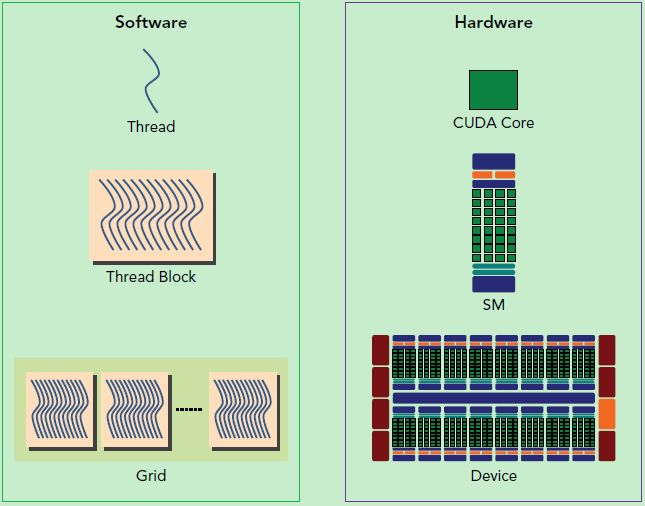
\includegraphics[width=0.7\textwidth]{image/1.3.1.q1.jpeg}
  \caption{Q1 示意图}
\end{figure}


\subsection{MPI}



\subsection{Pytorch}
\textbf{Q1.} \textit{nn.DataParallel (DP) 和 nn.parallel.DistributedDataParallel (DPP) 有什么区别?如何使用}

A1. 区别有一下几点:
\begin{itemize}
  \item DDP 通过\textbf{多进程}实现。操作系统会为每个 GPU 创建一个进程,从而过\textbf{避免了 Python 解释器 GIL 带来的性能开销}。而 DataParallel() 是通过单进程控制多线程来实现的;
  \item DDP 在各进程梯度计算完成之后,各进程需要将梯度进行汇总平均,然后再由 rank=0 的进程,将其 \textbf{broadcast 到所有进程后},各进程用该梯度来独立的更新参数。而 DP 是\textbf{梯度汇总到 GPU0},反向传播更新参数,再广播参数给其他剩余的 GPU;
  \item 相较于 DP, DDP 传输的数据量更少 (不需要广播模型参数),因此速度更快,效率更高。DDP 支持 all-reduce (指汇总不同 GPU 计算所得的梯度,并同步计算结果) ,broadcast, send 和 receive 等等。通过 MPI 实现 CPU 通信,通过 NCCL 实现 GPU 通信,缓解进程间通信带来的巨大开销问题;
  \item DDP 支持 SyncBN。SyncBN 即在数据并行分布式训练时,将各显卡上分配的数据汇总到一起进行规范化处理
\end{itemize}

\begin{lstlisting}
# DP 的使用
model = nn.DataParallel(model)

# DDP 使用
import torch
from torch.nn.parallel import DistributedDataParallel as DDP

torch.distributed.init_process_group(backend='nccl', world_size=ws, init_method='env://') # world_size 指的是总的并行进程数目,等到连接的进程数等于 world_size,程序才会继续运行
torch.cuda.set_device(local_rank) # 使用 local_rank 指定主机
device = torch.device(f'cuda:{local_rank}')
model = nn.Linear(2,3).to(device)
model = DDP(model, device_ids=[args.local_rank], output_device=args.local_rank).to(device)
\end{lstlisting}

\newpage


\section{工具类}

\begin{introduction}
\item Git
\item Linux
\item ROS
\end{introduction}

\subsection{Git}

\textbf{Q1.} \textit{如何修改前 n 次 commit,如果合并前 n 次 commit,如何修改已提交 commit?}

A1. 参考答案:

\begin{lstlisting}
# 修改前一次 commit
git commit --amend
# 修改前 n 次 commit
git rebase -i HEAD~n

# 合并前 n 次 commit
git reset --soft HEAD^n
git commit -m 'xxx'
# or
git rebase -i HEAD~n

# 修改已提交 commit,按照上述方法修改后,push
git push -f
\end{lstlisting}

\textbf{Q2.} \textit{如何回退到指定 commit?如果作者有打 tag,如何回退到指定 tag?}

A2. 参考答案:

\begin{lstlisting}
# 回退到指定 commit
git log # 查看 commit_message 和对应的 commit_id
git reset --hard commit_id

# 回退到指定 tag
git tag # 查看 tag
git checkout tag_name
\end{lstlisting}

\textbf{Q3.} \textit{如何给代码打 tag,如何给过去的 commit 打 tag?}

A3. 参考答案:

\begin{lstlisting}
# 给代码打 tag
git checkout master # 切换到要打 tag 的分支
git tag v1.0

# 给过去的 commit 打 tag
git log # 查看 commit_message 和对应的 commit_id
git tag v0.9 commit_id
\end{lstlisting}

\textbf{Q4.} \textit{简述流程:创建一个分支 dev,添加 readme.txt 文件,提交一次 commit 之后,merge 到 master 分支}

A4. 参考答案:

\begin{lstlisting}
git branch dev
git checkout dev
git add readme.txt 
git commit -m "add readme"
git checkout master
git merge dev
\end{lstlisting}


\subsection{Linux}

\textbf{Q1.} \textit{如何添加软链接,实现原理是什么?}

A1. ln -s。文件的储存是分为两部分的:inode 和 block。inode 存储了文件实际内容的指针,也就是文件的 block 的号码,以及其他诸如权限、日期等属性;block则是文件的具体内容。软链接指向文件名的 inode,根据文件名的 inode 最终读取到文件内容。\\

\subsection{ROS}

\newpage


\chapter{理论基础}

\section{机器学习和深度学习}

\begin{introduction}
\item Model Training
\item Efficient Network
\item Object Detection
\item Tracking
\item Segmentation
\item Person Re-ID
\end{introduction}

\subsection{Model Training}

\textbf{Q1.} \textit{过拟合常见的解决办法}

A1. 参考答案:

\begin{itemize}
  \item 增加数据,数据增强;
  \item Early stopping, Weight-decay, Dropout\\
\end{itemize}

\textbf{Q2.} \textit{列举常见的模型可视化算法。t-SNE 每次运行结果是一致的吗,为什么?t-SNE 中的近是真的近吗,远是真的远吗?}

A2. t-SNE 可视化特征分布,。t-SNE 本质上是基于流行学习 (manifold learning) 的降维算法,不同于传统的 PCA 和 MMD 等方法,t-SNE 在高维用 normalized Gaussian kernel 对数据点对进行相似性建模。相应的,在低维用t分布对数据点对进行相似性建模,然后用 KL 距离来拉近高维和低维空间中的距离分布。以及CAM 系列可视化 feature map,此处不再展开。

不一致。t-SNE 是在优化一个非凸的目标函数,我们每次得到的只不过是一个局部最小。

近是真的近,远不是真的远。对 t 分布来说,超出一定距离范围以后,其相似度都是很小的。也就是说,只要不在一个集群范围内,其相似度都是一个很小的值。\\


\textbf{Q3.} \textit{简述 k-means 的算法流程}

A3. 参考答案:

\begin{itemize}
  \item 选择初始化的 k 个样本作为初始聚类中心 $a={a_1,a_2,…a_k}$;
  \item 针对数据集中每个样本 $x_i$ 计算它到 k 个聚类中心的距离并将其分到距离最小的聚类中心所对应的类中;
  \item 针对每个类别 $a_j$,重新计算它的聚类中心 $a_j=\frac{1}{\left| c_i \right|}\sum_{x\in c_i}x$ (即属于该类的所有样本的质心);
  \item 重复上面 2、3 两步操作,直到达到某个中止条件 (迭代次数、最小误差变化等)。\\
\end{itemize}


\textbf{Q4.} \textit{Batch Normalization,Instance Normalization,Layer Normalization 和 Group Normalization 分别如何计算}

A4. 将输入图像的 shape 记为 [N, C, H, W],则这几个方法:
\begin{itemize}
  \item Batch Normalization 是在 batch 维度上,对 NHW 做归一化;
  \item Layer Normalization 在通道方向上,对 CHW 归一化;
  \item Instance Normalization 在图像像素维度上,对 HW 做归一化;
  \item GroupNorm 将 channel 分组,然后再做归一化
\end{itemize}

具体可见下图

\begin{figure}[ht]
  \centering
  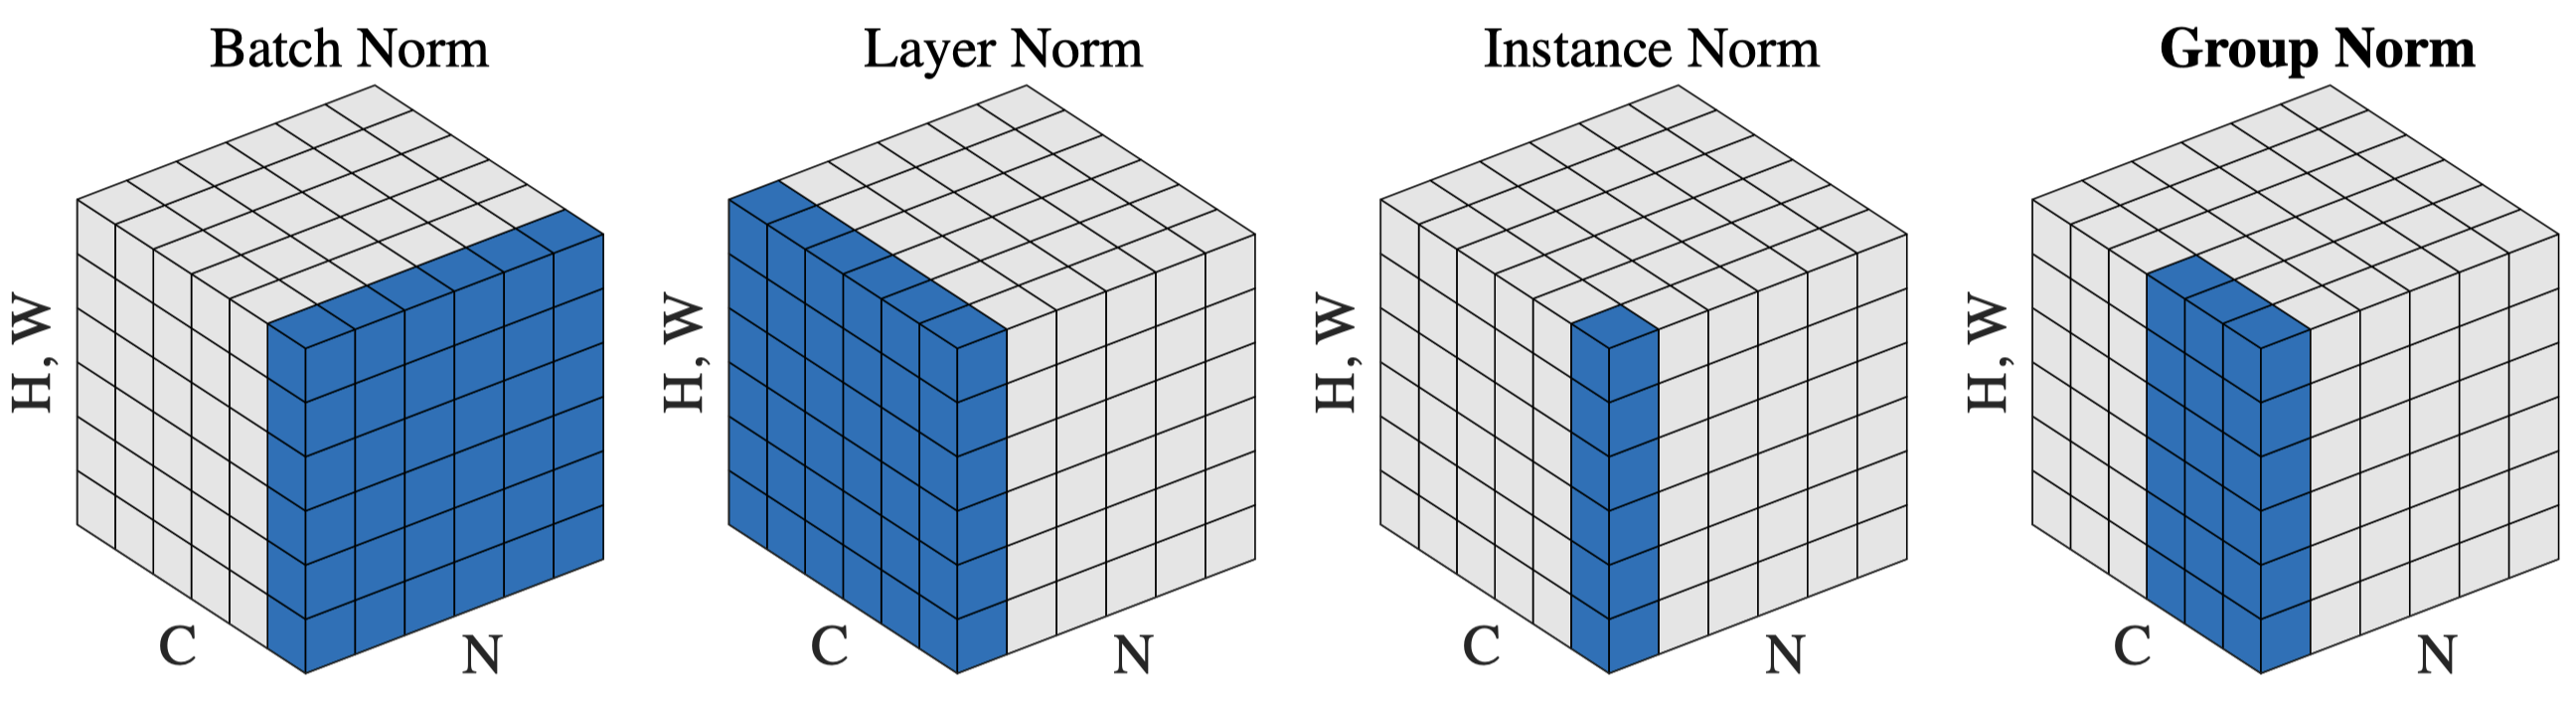
\includegraphics[width=0.7\textwidth]{image/2.1.1.q4.png}
  \caption{2.1.1.Q4 示意图}
\end{figure}
 
\subsection{Efficient Network}

\textbf{Q1.} \textit{衡量效率的指标有哪些,如何计算?}

A1. 参考答案:
\begin{itemize}
  \item FLOPS:floating point operations per second,指每秒浮点运算次数,理解为计算速度。是一个衡量硬件性能的指标;
  \item FLOPs:floating point operations ,指浮点运算数,理解为计算量。可以用来衡量算法/模型的复杂度;
  \item MAC:Memory Access Cost,计算机在进行计算时候要加载到缓存中,然后再计算,这个加载过程是需要时间的。其中,分组卷积 (group convolution) 是对 MAC 消耗比较多的操作 (因此 ShuffleNet V2 取消了 group convolution)\\
\end{itemize}


\textbf{Q2.} \textit{模型压缩的主要方法有哪些?}

A2. 参考答案:

\begin{itemize}
  \item 从模型结构上优化:模型剪枝、模型蒸馏、automl 直接学习出简单的结构;
  \item 模型参数量化将 FP32 的数值精度量化到 FP16、INT8、二值网络、三值网络等\\
\end{itemize}


\textbf{Q3.} \textit{Depthwise separable convolution 运算过程,为什么能节省计算量?}

A3. 以分组卷积为基础,深度可分离卷积的第一步是分组为 $C_{in}$ 的分组卷积。这个过程中,对于输入特征图的每个通道,通过一个尺寸为 $K\times{K}$ 的卷积核,计算结果作为输出特征图的一个通道,不进行通道数的增加和减少。然后通过逐点卷积 (Pointwise Convolution) 实现通道数改变,这个过程使用大小为 $C_{in} \times {1} \times {1}$ 的卷积核实现,输出通道数为 $C_{out}$ 个。深度可分离卷积所需参数量为:$C_{in}\times{K}\times{K}+C_{in}\times{1}\times{1}\times{C_{out}}$。

下图为 Depthwise separable convolution 示意图:

\begin{figure}[ht]
  \centering
  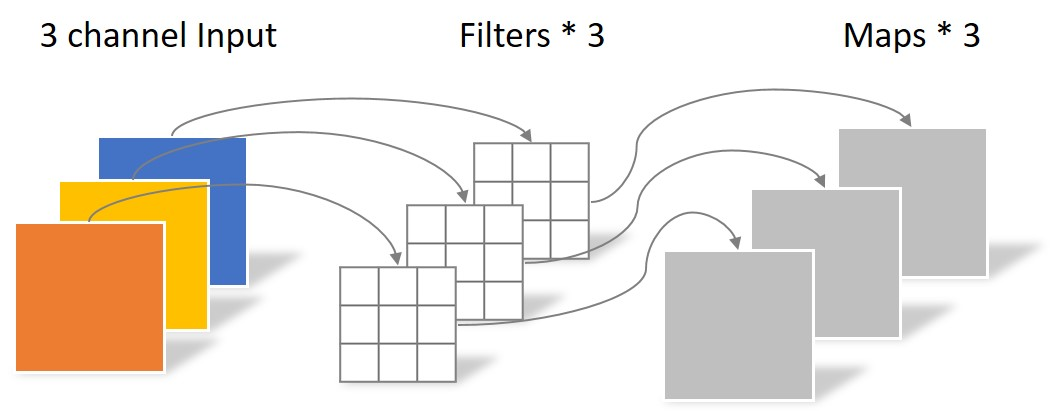
\includegraphics[width=0.8\textwidth]{image/2.1.2.q3.jpeg}
  \caption{2.1.2.Q3 示意图}
\end{figure}


\subsection{Object Detection}

\textbf{Q1.} \textit{分别介绍 Anchor-based 和 Anchor-free 有哪些主流方法?基于 Faster R-CNN、CenterNet 介绍 Anchor-based 和 Anchor-free 的 pipeline}

A1. Anchor-based 的方法分为 one-stage 和 two-stage,one-stage 有 RetinaNet、YOLO 系列 (除 v1)、SSD 等,two-stage 有 Faster R-CNN、Cascade R-CNN、Mask R-CNN 等。Anchor-free 的方法有 CenterNet、CornerNet、FCOS、RepPoints 等。\\


\textbf{Q2.} \textit{RoIAlign 解决了什么问题,具体是如何实现的?}

A2. 解决 RoIPooling 中两次量化取整的精度损失。具体是使用双线性插值。

RoIPooling 的两次量化误差如下图所示:

\begin{figure}[ht]
\centering
    \subfigure[Feature map 取整]{
    \begin{minipage}[t]{0.5\linewidth}
    \centering
    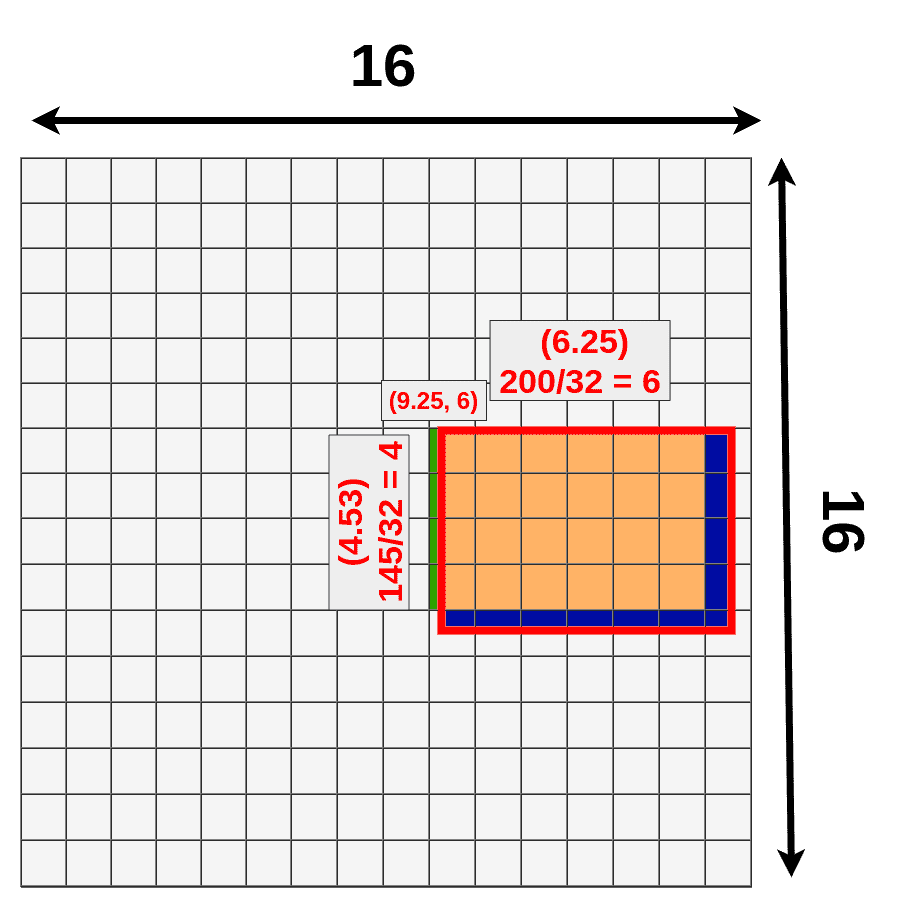
\includegraphics[width=0.8\linewidth]{image/2.1.3.q2.1.png}
    % \caption{feature map 取整}
    \end{minipage}%
    }%
    \subfigure[Pooling 时取整]{
    \begin{minipage}[t]{0.5\linewidth}
    \centering
    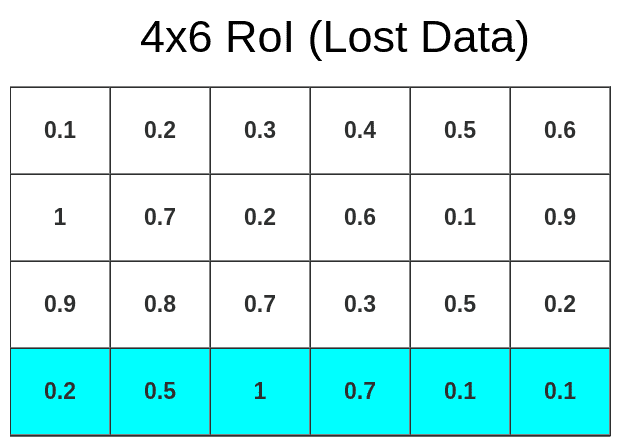
\includegraphics[width=0.9\linewidth]{image/2.1.3.q2.2.png}
    % \caption{Pooling 时取整}
    \end{minipage}%
    }%
\centering
\caption{2.1.3.Q2.1 示意图}
\end{figure}

RoIAlign 过程如下图所示,对特征图进行双线性插值,然后在浮点数的坐标上采样:
\begin{figure}[ht]
  \centering
  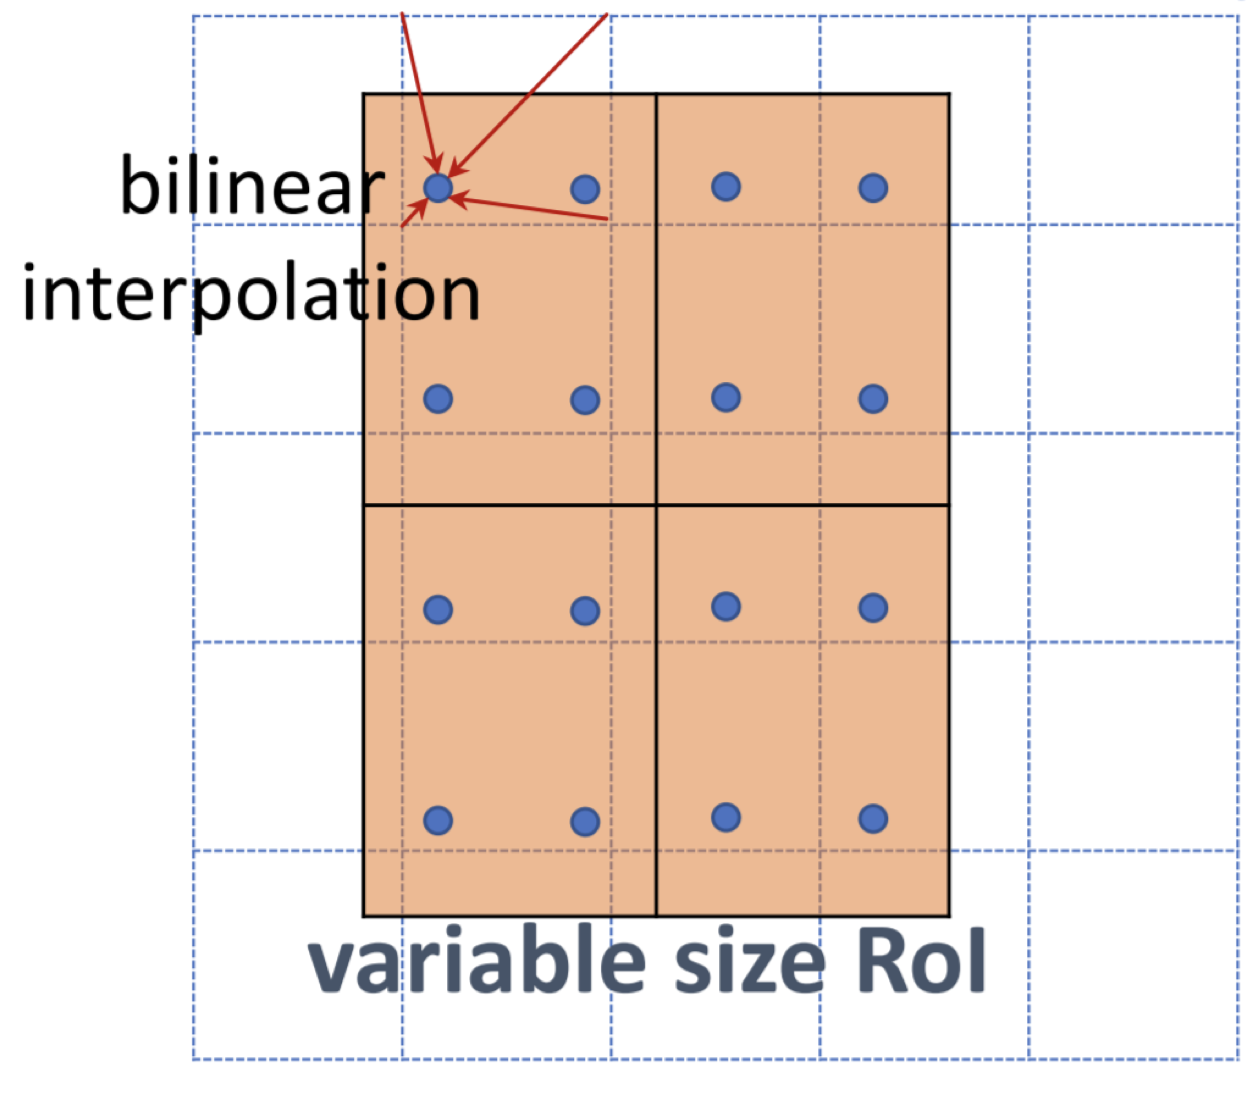
\includegraphics[width=0.35\textwidth]{image/2.1.3.q2.3.png}
  \caption{2.1.3.Q2.2 示意图}
\end{figure}


\textbf{Q3.} \textit{NMS 中存在什么问题?有哪些变体?}

A3. NMS 存在以下缺点:
\begin{itemize}
  \item 将得分较低的边框强制性地去掉,如果物体出现较为密集时,本身属于两个物体的边框,其中得分较低的也有可能被抑制掉,降低了模型的召回率;
  \item NMS 的实现存在较多的循环步骤,GPU 的并行化实现不是特别容易,尤其是预测框较多时,耗时较多;
  \item 将得分作为衡量指标。NMS 简单地将得分作为一个边框的置信度,但在一些情况下,得分高的边框不一定位置更准。阈值难以确定。过高的阈值容易出现大量误检,而过低的阈值则容易降低模型的召回率,超参很难确定
\end{itemize}


变体一:Soft NMS。对于 IoU 大于阈值的边框,没有将其得分直接置 0,而是降低该边框的得分。降低的公式为:

\begin{equation}
s_{i}=s_{i} e^{-\frac{\operatorname{iou}\left(\mathcal{M}, b_{i}\right)^{2}}{\sigma}}, \forall b_{i} \notin \mathcal{D}
\end{equation}

变体二:Adaptive NMS。通过网络预测目标周边的密集和稀疏的程度,采用不同的去重策略。在人群密集的地方,NMS 阈值较大,而人群稀疏的地方 NMS 阈值较小。具体来说,首先定义 density:

\begin{equation}
d_{i}:=\max _{b_{j} \in \mathcal{G}, i \neq j} \operatorname{iou}\left(b_{i}, b_{j}\right)
\end{equation}

然后改进 Soft NMS 为:
\begin{equation}
\begin{gathered}
N_{\mathcal{M}}:=\max \left(N_{t}, d_{\mathcal{M}}\right), \\
s_{i}= \begin{cases}s_{i}, & \operatorname{iou}\left(\mathcal{M}, b_{i}\right)<N_{\mathcal{M}} \\
s_{i} f\left(\operatorname{iou}\left(\mathcal{M}, b_{i}\right)\right), & \operatorname{iou}\left(\mathcal{M}, b_{i}\right) \geq N_{\mathcal{M}}\end{cases}
\end{gathered}
\end{equation}


\textbf{Q4.} \textit{FPN 有哪些变体,他们被提出的动机分别是什么?}

A4. 有以下变体
\begin{itemize}
  \item PANet。FPN 没有很好地利用低层信息,PANet 增加了 Bottom-up Path Augmentation,将低层的信息又传导到高层中去,同时减少了高层到低层的信息流通需要穿过的卷积层数;
  \item BiFPN。改进了 PANet,结构相似。BiFPN 寻找了一个有效的 block,然后 repeat 的次数是可以调节的超参;
  \item NAS-FPN。设计搜索空间来发现新的 FPN 结构。这种 FPN 可以重复堆叠,并且与 BiFPN 相比连接更少;
  \item Recursive-FPN。见下图
\end{itemize}

\begin{figure}[ht]
  \centering
  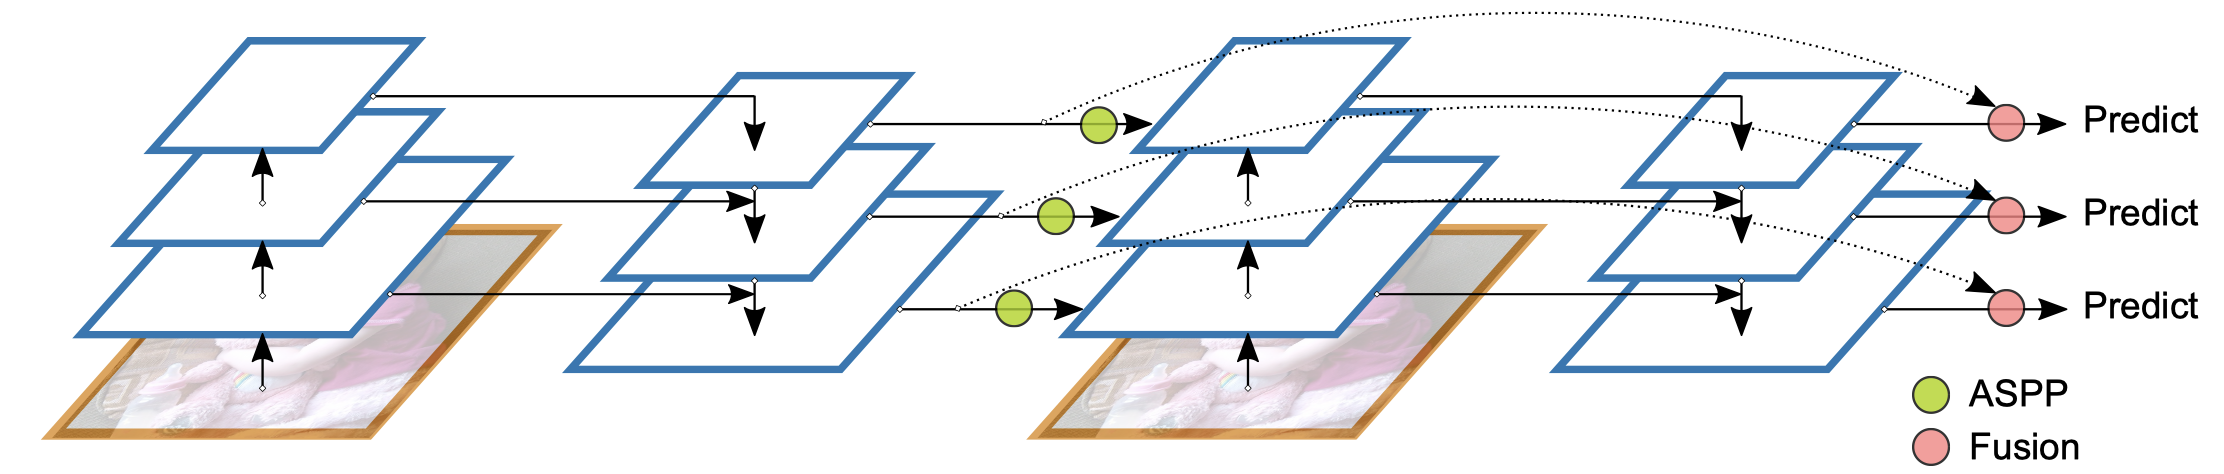
\includegraphics[width=0.8\textwidth]{image/2.1.3.q4.png}
  \caption{2.1.3.Q4 示意图}
\end{figure}


\subsection{Tracking}

\subsection{Segmentation}

\subsection{Person Re-ID}

\textbf{Q1.} \textit{Re-ID 中常用的 mAP 指标如何计算?}

A1. 对于一张 query,$AP$ 的计算方式:

\begin{equation}
AP(q)=\frac{\sum_{k} P(k) \times \delta_{k}}{N_{g t}(q)}
\end{equation}

$P(k)$ 代表在 rank k 时的 precision,$N_{g t}(q)$ 是该 query 在 gallery 中出现总次数,当 rank k 命中时 $\delta_{k}=1$. $mAP$ 是所有 query images 上 $AP$ 的均值:

\begin{equation}
mAP=\frac{\sum_{q} AP(q)}{Q}
\end{equation}

\textbf{Q2.} \textit{Softmax loss 的公式。在 Re-ID 中还有那些常用的变体?}

A2. 

\begin{equation}
l= -\log z_k=-\log \frac{e^{l_k}}{\sum_{i=1}^{C}{e^{l_i}}}=-\log \frac{e^{x^T·\omega_k+b_k}}{\sum_{i=1}^{C}{e^{x^T·\omega_i+b_i}}} \\
\end{equation}

变体中最常用的是 cosface。cosface 对 $W$ 和 $x$ 做归一化,然后直接在余弦空间中最大化分类界限,即对余弦值添加一个 margin 项 $m$:

\begin{equation}
L_{l m c}=\frac{1}{N} \sum_{i}-\log \frac{e^{s\left(\cos \left(\theta_{y_{i}, i}\right)-m\right)}}{e^{s\left(\cos \left(\theta_{y_{i}, i}\right)-m\right)}+\sum_{j \neq y_{i}} e^{s \cos \left(\theta_{j, i}\right)}}
\end{equation}

% \textbf{Q3.} \textit{Triplet loss 的公式。在 Re-ID 中还有那些常用的变体?}

% A3. 

% \textbf{Q4.} \textit{介绍一下 part-based 的方法 PCB}

% A4. 


% \textbf{Q5.} \textit{介绍一种 re-ranking 算法}

% A5. 


\newpage


\section{计算机图形学}

\begin{introduction}
\item 色彩空间
\item ISP
\item 常见图像处理算法及 OpenCV 实现
\end{introduction}

\subsection{色彩空间}

\subsection{ISP}

\textit{ISP 的 pipeline 通常包括哪些操作?}

A1. 列表与图片不一定完全对应,不同硬件的 pipeline 也不完全相同,能回答出大部分即可。

\begin{itemize}
  \item Input Signal: 输入数字后端的信号模态是数字信号,单通道的 RAW 格式;
  \item BLC (Black Level Correction):Black Level定义为“无图像状态时的电平”。因为器件存在暗电流,此电平信号并不是 0,故需要用部分不感光的区域对电流敏感性进行矫正;
  \item BPC (Bad Point Correction):因为制作工艺而导致个别像素点出现“无电流、恒高电流、电流漂移”等特性,常用邻域法;
  \item GIC (Green Imbalance Correction):Bayer 玻片的两个 G 通道,临近 R 和 B,因此两个 G 工艺可能存在差异,进而导致 Gr 和 Gb 通道获得能量有差异。此原因一般为:a. 半导体工艺差异。b. 传感器前端的 micro lense 对图像边缘的影响。Gr 和 Gb 通道差异最有可能放大高频过渡带,导致图像产生格子迷宫;
  \item LSC (Lens Shading Correction):镜头的光灵敏度在趋近视野边缘会逐渐降低。灵敏度的下降是 $cos^{4}\theta$ 趋势下降的,因此补偿方式就是用灵敏度曲线作为补偿因子,补偿四周的亮度值;
  \item Demosaic:光从进入 CMOS 前要通过 Bayer 滤波片 (CFA),图像进入数字后端后是 RAW 域的昏暗图像。Demosaic 模块就是通过插值,将单颜色通道图像恢复成人眼识别的 RGB 图像,最常见的插值方式就是邻域/双线性插值;
  \item AWB (Automatic White Balance):相机成像受光源颜色的影响很大,需要动态获得场景内的白点。确定白点的方式通常为:a). 场景内平均颜色为灰度的中值,计算白点;b). 最亮处为白点 c). 捕捉到色彩的分布来评估光源。通常为三种混合使用;
  \item CCM (Color Correction Matrix):RGB 矫正是避免图像传感器颜色滤波中的溢出现象。方法是,先拍摄一幅图像,和标准图像比对后,计算出矫正矩阵,{a,b,c} 是标准化的单位矩阵,矫正过程如图4所示,通常会影响图像的饱和度;
  \item GC (Gamma Correction):在模拟前端,光信号转换为电信号的过程存在很多非线性变换。这一类非线性函数都可以近似为 $\gamma$ 幂函数形式。通过幂函数对非线性函数进行线性矫正的过程,称为伽马矫正。通常,$\gamma$ 值是需要根据设备和场景调节的。当 $\gamma > 1$ 时,低照度被拓展,高亮度被压缩;反之亦然;
  \item Distortion Remove:由于镜头总存在角度的失真,图像和真实场景不能实现完美映射。常见的空间畸变为两类,桶形畸变和枕形畸变。去畸变模块是为了实现空间的一对一映射;
  \item Sharpen:锐化可以增强图像纹理细节,但是高频噪声也会被增强;
  \item YUV Transform:除了 RGB 域图像,另一类图像表示方式是 YUV 域。YUV 图像的优势是:低存储性,便于传输。该方式利用了人眼对亮度的敏感性高于色度,用 Y 通道表示明亮度,就是灰阶值。U 和 V 通道表示色度;
  \item AE (Automatic Exposure):AE 可以让照相机模拟人眼的光强适应能力。通过调整入射光量,从而充分利用其动态范围。实现方式通常是先将图像分割为自动曝光窗口,通过计算每个窗口内的信号的平均值、方差和峰值,以确定量化指标光亮度,最终调节曝光时间。最终实现图像质量不受光线微弱变化造成的影响
\end{itemize}

\begin{figure}[h]
  \centering
  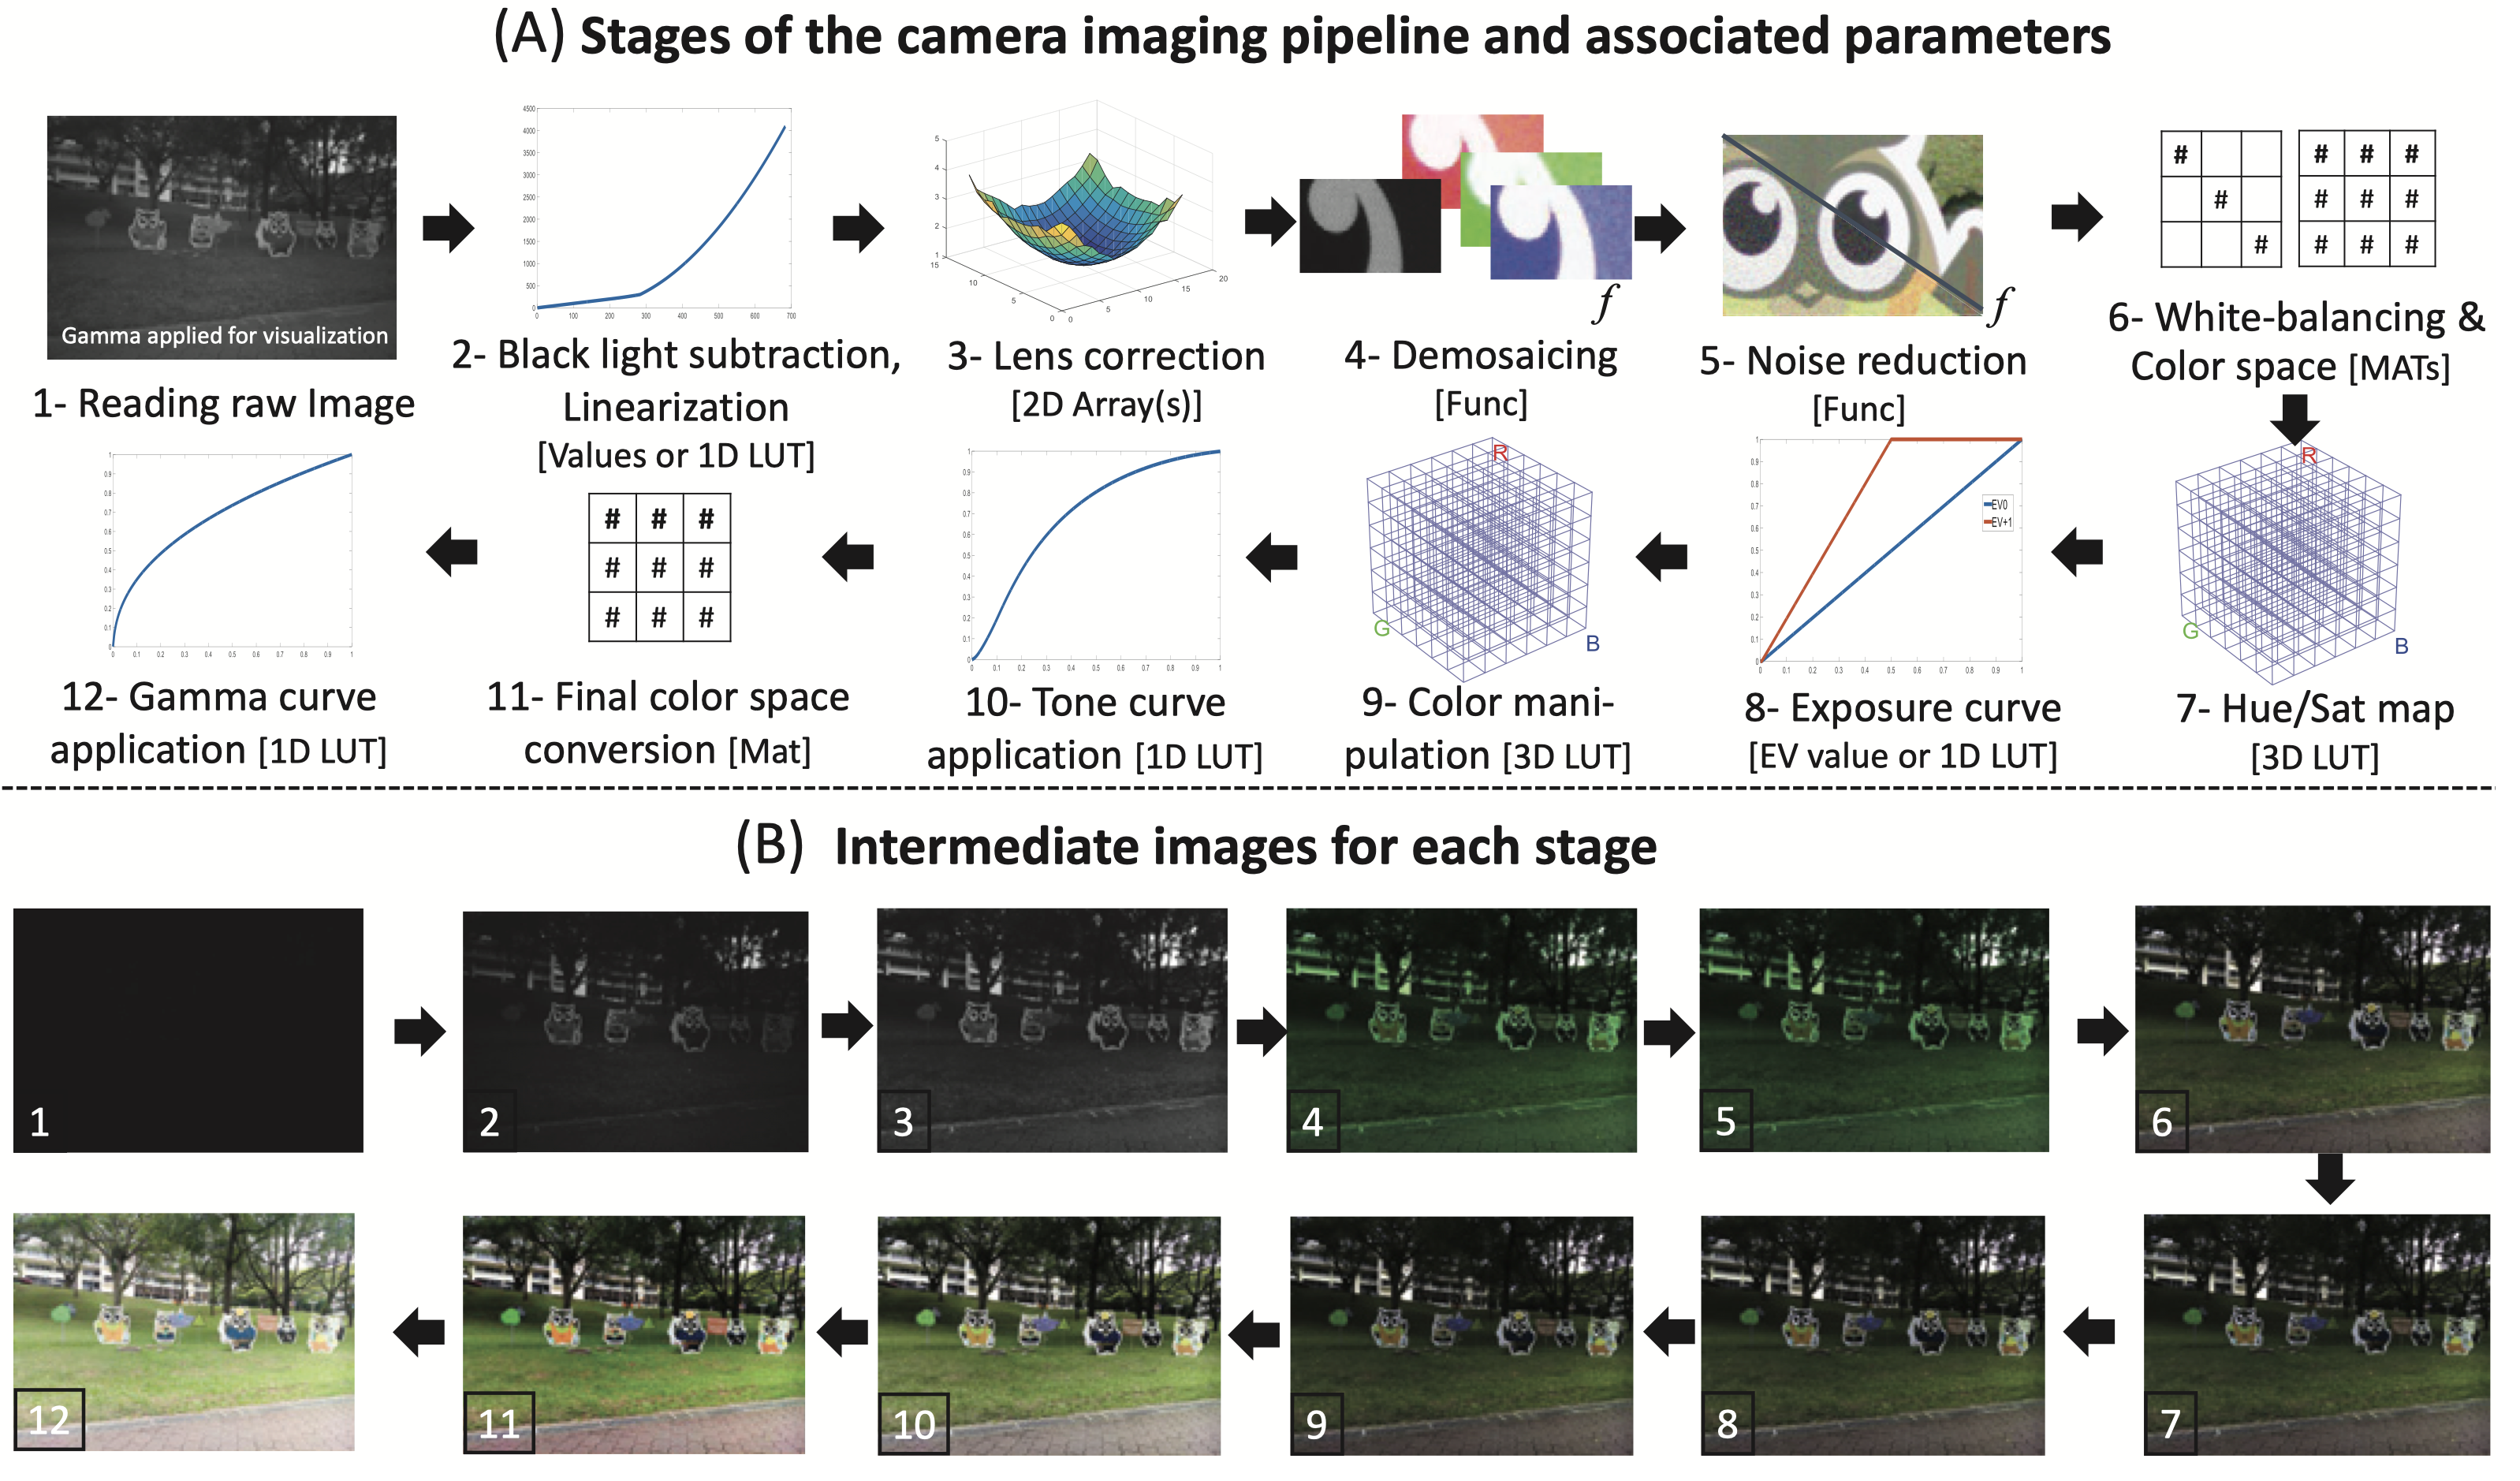
\includegraphics[width=0.9\textwidth]{image/2.2.2.q1.png}
  \caption{Q1 示意图}
\end{figure}


\subsection{常见图像处理算法及 OpenCV 实现}

\textbf{Q1.} \textit{什么是均值滤波,中值滤波,高斯滤波。写出高斯滤波的 kernel。}

A1. 均值滤波:用像素点周围像素的平均值代替原像素值,其在过滤噪声的同时也会过滤掉图像的边缘信息。在 OpenCV 中,使用 boxFilter() 和 blur() 函数进行均值滤波。均值滤波 kernel 如下所示:

\begin{equation}
k=\frac{1}{K_{\text {width }} \cdot K_{\text {height }}}\left(\begin{array}{ccc}
1 & \cdots & 1 \\
\vdots & \ddots & \vdots \\
1 & \cdots & 1
\end{array}\right)
\end{equation}

中值滤波:用像素点周围像素的中值代替原像素值,中值滤波对于消除图像中的椒盐噪声十分有效。在 OpenCV 中,使用 medianBlur() 函数进行中值滤波。

高斯滤波:与均值滤波原理类似,用像素点周围像素的均值代替原像素值。但其 kernel 的系数与均值滤波不同,高斯滤波 kernel 的系数则随着距离中心位置的增大而减小。一个二维高斯函数如下所示,其中,$(k, l)$ 为 kernel 的中心坐标,$(i, j)$ 为 kernel 其它系数的坐标,$\sigma$ 为高斯函数的标准差。相比于均值滤波,高斯滤波会减弱图像的模糊程度。在 OpenCV 中,使用 GaussianBlur() 函数进行高斯滤波。

\begin{equation}
d(i, j, k, l)=e^{-\frac{(i-k)^{2}+(j-l)^{2}}{2 \sigma^{2}}}
\end{equation}


\newpage


\section{数学基础}

\begin{introduction}
\item 概率论
\item 矩阵论
\item 高等数学
\end{introduction}

\subsection{概率论}

\textbf{Q1.} \textit{圆上任取三点,构成锐角三角形的概率。}

A1. 假设圆半径为 1。首先固定住 A 点,我们把 A 点作为三角形的第一个点。接下来在圆周取作为三角形第二个点的点 C。点 C 可能在 AB 的左边,也可能在 AB 的右边。由于左右完全对称,因此不妨设点 C 在 AB 的左边。

\begin{figure}[ht]
  \centering
  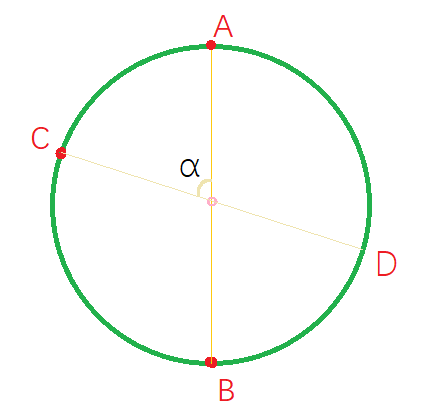
\includegraphics[width=0.4\textwidth]{2.3.1.q1.png}
  \caption{Q1 示意图}
\end{figure}

最后一步是三角形第三个点的选取。易知,只有当第三个点E在劣弧BD上时,ACE才能组成锐角三角形(一个事实是:圆周上三个点组成锐角三角形,当且仅当圆心在三角形内部)。此时的概率为 $\frac{\tilde{BD}}{2\pi}=\frac{\alpha}{2\pi}$,其中 $\tilde{BD}$ 表示劣弧 $BD$ 的弧长。

我们知道 $\alpha$ 服从 $(0,\pi)$ 上的均匀分布,经过加权得(即运用全概率公式):

\begin{equation}
\int_{0}^{\pi}\frac{\alpha}{2\pi}\cdot\frac{1}{\pi}d\alpha=\frac{1}{4}
\end{equation}

\textbf{Q2.} \textit{抛一枚均匀的硬币若干次,直到出现连续两次正面向上,所需抛硬币总次数的数学期望是多少?}

A2. 首先设连续两次正面的期望次数为 $x$。1 次正面的期望次数为 $2$。接下来有 $\frac{1}{2}$ 的概率再出现正面,这时抛币次数为 $2+1$。有 $\frac{1}{2}$ 的概率再出来一个反面,这时总期望次数为 $2+1+x$。所以:

\begin{equation}
x=1/2 * (2+1) + 1/2 * (2+1+x)
\end{equation}

解得 $x=6$。\\


\subsection{矩阵论}

\subsection{高等数学}

\textbf{Q1.} \textit{$a$ 和 $b$ 满足在 $[0, 1]$ 上均匀分布,求 $max(a, b)$ 的期望值。}

A1. 均匀分布的概率密度函数为:
\begin{equation}
f(x)= \begin{cases}\frac{1}{b-a}, & a<x<b \\ 0, & \text { else }\end{cases}
\end{equation}

因为 a, b 独立,所以二维随机变量 (a, b) 的概率密度函数为:
\begin{equation}
f(a, b)=f(a) f(b)=\frac{1}{(1-0)^{2}}
\end{equation}

根据期望值公式可以得到:
\begin{equation}
E(\max (a, b))=\int-\infty^{+\infty} \int-\infty^{+\infty} \max (a, b) f(a, b) d a d b
\end{equation}

$a>b$ 与 $a<b$ 的情况对称,不妨设 $a>b$。则期望值为:
\begin{equation}
E(\max (a, b))=E(a)=\int_{0}^{1} d a \int_{0}^{a} a d b=\frac{1}{3}
\end{equation}

因此最终答案是 $\frac{2}{3}$


\newpage


\section{SLAM}

\textbf{Q1.} \textit{视差与深度的关系,建议候选人通过绘图的方式答题}

A1. 距离像面越近的点,它在左右相机中的视差越大,距离像面越远的点,它在左右相机中的视差越小。


\textbf{Q2.} \textit{描述一下极线约束,建议候选人通过绘图的方式答题}

A2. 极线约束描述的是当同一个点投影到两个不同视角的图像上时,像点、相机光心在投影模型下形成的约束。


\begin{figure}[ht]
  \centering
  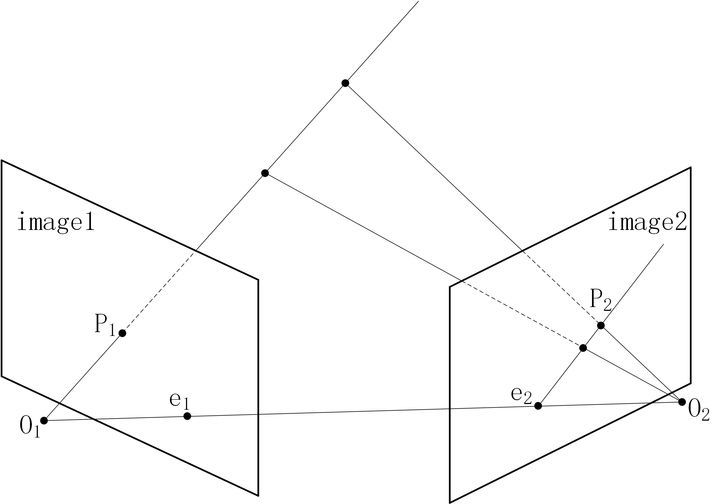
\includegraphics[width=0.6\textwidth]{image/2.4.q2.jpeg}
  \caption{Q2 示意图}
\end{figure}


已知,相机 1 和相机 2 的内参矩阵分别为 $K_1$、$K_2$,坐标系 1 与坐标系 2 的外参为 $R$、$t$,世界点 P 在 image1 上的像点为 $P_1(u_1,v_1,1)$。假设,世界点 P 在 image2 上的像点为 $P_1(u,v,1)$。 第一步,将所有点变换到相机 2 坐标系:


\begin{equation}
\begin{gathered}
P_{c 1}=\left(\begin{array}{l}
x_{c 1} \\
y_{c 1} \\
z_{c 1}
\end{array}\right)=R(K_{1}^{-1}\left(\begin{array}{c}
u_{1} \\
v_{1} \\
1
\end{array}\right))+t \\
P_{c 2}=\left(\begin{array}{l}
x_{c 2} \\
y_{c 2} \\
z_{c 2}
\end{array}\right)=K_{2}^{-1}\left(\begin{array}{c}
u \\
v \\
1
\end{array}\right)
\end{gathered}
\end{equation}


所以,平面 $O_1O_2P$ 的法向量在相机 2 的相机坐标系中为:


\begin{equation}
\vec{n}=t \times p_{c 1}=t^{T T} p_{c 1}
\end{equation}


$t^{TT}$ 为平移向量 $t$ 的反对称矩阵。法向量 $\vec{n}$ 与向量 $P_{c2}$ 垂直,即:


\begin{equation}
p_{c 2}^{T} \cdot \vec{n}=0
\end{equation}


将上式带入整理得:


\begin{equation}
\left(\begin{array}{lll}
u & v & 1
\end{array}\right) K_{2}^{-T} \cdot t^{T T} R \cdot K_{1}^{-1}\left(\begin{array}{c}
u_{1} \\
v_{1} \\
1
\end{array}\right)=0
\end{equation}


这个式子就是极线 $e_2P_2$ 的直线方程。另外,$t^{TT}R$ 被称为本征矩阵(Essential Matrix),$K_2^{-T} \cdot   t^{TT}R\cdot K_1^{-1}$ 被称为基础矩阵(Fundamental Matrix)。\\


\textbf{Q3.} \textit{基础矩阵 (Fundamental Matrix)、本质矩阵 (Essential) 和单应矩阵 (Homography) 的区别,自由度分别为多少?}


A3. 基础矩阵是任意两个相机相对关系的内参,换言之,给定了两个相机的相对位置关系和相机内参,基础矩阵即被确定。首先 F 矩阵是三阶的,最高自由度为 9,然后其满足尺度等价性 (因为图像坐标是通过齐次坐标表示,因此你矩阵同乘一个常数,最后求得的坐标其实是一致的,可以理解为 $H_{33}$ 衡等于 1,或者满足一个约束等式),因此自由度减一,再其次其满足不可逆矩阵的性质,行列式为零的约束等式,因此自由度再减一,为 7。


\begin{figure}[ht]
  \centering
  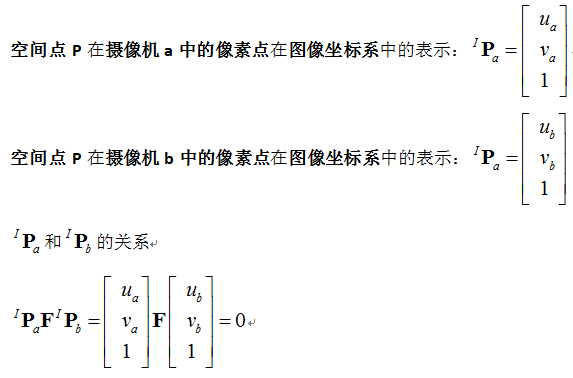
\includegraphics[width=0.6\textwidth]{image/2.4.q3.1.png}
  \caption{Q3 示意图 1}
\end{figure}


本质矩阵是两个标准相机相对关系的内参,换言之,给定两个已标定相机的相对位置关系,本质矩阵即被确定。本质矩阵是归一化坐标系下基础矩阵的特殊形式。由此可得,本质矩阵 (E 矩阵) 平移 $t$ 的待自由度是 3 ($xyz$ 三个方向),旋转矩阵 $R$ 的自由度是 3 (row,pitch,yaw 三个方向),所以其自由度最高是 6,同时 $E$ 满足尺度等价性约束,所以 $E$ 的自由度减一,其自由度为 5。


\begin{figure}[ht]
  \centering
  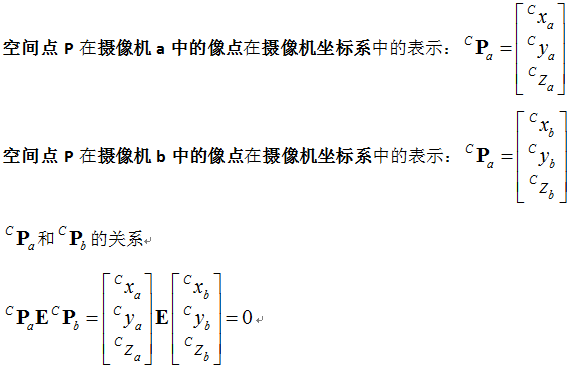
\includegraphics[width=0.6\textwidth]{image/2.4.q3.2.png}
  \caption{Q3 示意图 2}
\end{figure}


单应矩阵所有的空间点都再同一个平面上,则两幅图像中的点都满足同一个射影变换,该射影变换即单应矩阵,射影变换的自由度为 9,其同样具有尺度等价性 (因为图像坐标是通过齐次坐标表示,因此你矩阵同乘一个常数,最后求得的坐标其实是一致的),因此自由度减一,其自由度为 8。\\


\textbf{Q4.} \textit{闭环检测常用方法}

A4. ORB SLAM 中采用的是词袋模型进行闭环检测筛选出候选帧,再通过求解 Sim3 判断最合适的关键帧。

LSD SLAM 中的闭环检测主要是根据视差、关键帧连接关系,找出候选帧,然后对每个候选帧和测试的关键帧之间进行双向 Sim3 跟踪,如果求解出的两个李代数满足马氏距离在一定范围内,则认为是闭环成功。\\


\textbf{Q5.} \textit{什么是 PnP 问题,你了解哪些解法?}

A5. 参考:\hyperlink{https://zhuanlan.zhihu.com/p/399140251}{\textcolor{blue}{PnP (Perspective-n-Point) 问题:各种算法总结分析}} 

PnP (Perspective-n-Point) 是求解 3D 到 2D 点对运动的方法,目的是求解相机坐标系相对世界坐标系的位姿。它描述了已知 $n$ 个 3D 点的坐标 (相对世界坐标系) 以及这些点的像素坐标时,如何估计相机的位姿 (即求解世界坐标系到相机坐标系的旋转矩阵 $R$ 和平移向量 $t$)。

算法:直接线性变换 (DLT)、P3P、EPnP、光束法平差 (BA,Bundle Adjustment)。\\


\textbf{Q6.} \textit{单目视觉 SLAM 中尺寸漂移是怎么产生的,如何修正?}

A6. 用单目估计出来的位移,与真实世界相差一个比例,叫做尺度。这个比例在单目初始化时通过三角化确定,但单纯靠视觉无法确定这个比例到底有多大。由于SLAM过程中噪声的影响,这个比例还不是固定不变的。修正方式是通过回环检测计算 Sim3 进行修正。\\


\textbf{Q7.} \textit{介绍你熟悉的边缘检测算子}

A7. 边缘检测一般分为三步,分别是滤波、增强、检测。基本原理都是用高斯滤波器进行去噪,之后在用卷积内核寻找像素梯度。常用有三种算法:canny 算子,sobel 算子,laplacian 算子

canny 算子:一种完善的边缘检测算法,抗噪能力强,用高斯滤波平滑图像,用一阶偏导的有限差分计算梯度的幅值和方向,对梯度幅值进行非极大值抑制,采用双阈值检测和连接边缘。

sobel 算子:一阶导数算子,引入局部平均运算,对噪声具有平滑作用,抗噪声能力强,计算量较大,但定位精度不高,得到的边缘比较粗,适用于精度要求不高的场合。

laplacian 算子:二阶微分算子,具有旋转不变性,容易受噪声影响,不能检测边缘的方向,一般不直接用于检测边缘,而是判断明暗变化。\\


\textbf{Q8.} \textit{3D 空间的位姿如何去表达?}

A8. 李群或李代数。\\


\textbf{Q9.} \textit{给两组已经匹配好的 3D 点,如何计算相对位姿变换,写出伪代码}

A9. ICP (Iterative Closest Point)。ICP 的解法一共有两种:SVD 方法和非线性优化方法。SVD 解法参考 \hyperlink{https://zhuanlan.zhihu.com/p/111933242}{\textcolor{blue}{ICP 的 SVD 解法}}\\


\textbf{Q10.} \textit{ORB-SLAM 初始化的时候为什么要同时计算 H 矩阵和 F 矩阵}

A10. 简单地说,因为初始化的时候如果出现纯旋转或者所有特征点在同一个平面上的情况,F 矩阵会发生自由度退化,而这个时候 H 矩阵会有较小误差,因此要同时计算 H 矩阵和 F 矩阵。\\


\textbf{Q11.} \textit{给一张图片,知道相机与地面之间的相对关系,如何计算出图的俯视图。}

A11. (1)灰度化处理;(2)滤波处理;(3)边缘检测;(4)寻找四个点——霍夫变换直线识别;(5)计算 H 矩阵;(6)消除透视失真。\\


\chapter{在线编程}

\section{LeetCode 编程题}

\textbf{Q1.} \textit{合并两个有序数组}

给你两个按非递减顺序 排列的整数数组 $nums1$ 和 $nums2$,另有两个整数 $m$ 和 $n$ ,分别表示 $nums1$ 和 $nums2$ 中的元素数目。请你合并 $nums2$ 到 $nums1$ 中,使合并后的数组同样按非递减顺序排列。

你可以设计实现一个时间复杂度为 $O(m + n)$ 的算法解决此问题吗?

\textbf{测试用例}:
\begin{lstlisting} [language=python]
输入:nums1 = [1,2,3], m = 3, nums2 = [2,5,6], n = 3
输出:[1,2,2,3,5,6]

输入:nums1 = [1], m = 1, nums2 = [], n = 0
输出:[1]

输入:nums1 = [20, 12, 43, 13, 11], m = 5, nums2 = [2, 4, 1, 5], n = 4
输出:[1, 2, 4, 5, 11, 12, 13, 20, 43]
\end{lstlisting}


\textbf{参考思路}:将两个数组合并再排序则合格,使用双指针则优秀。双指针参考:

\begin{lstlisting} [language=python]
class Solution:
    def merge(self, nums1: List[int], m: int, nums2: List[int], n: int) -> List[int]:
        sorted = []
        p1, p2 = 0, 0
        while p1 < m or p2 < n:
            if p1 == m:
                sorted.append(nums2[p2])
                p2 += 1
            elif p2 == n:
                sorted.append(nums1[p1])
                p1 += 1
            elif nums1[p1] < nums2[p2]:
                sorted.append(nums1[p1])
                p1 += 1
            else:
                sorted.append(nums2[p2])
                p2 += 1
        return sorted
\end{lstlisting}


\textbf{Q2.} \textit{Two Sum}

给定一个整数数组 $nums$ 和一个整数目标值 $target$,请你在该数组中找出和为目标值 $target$ 的那两个整数,并返回它们的数组下标。

你可以假设每种输入只会对应一个答案。但是,数组中同一个元素在答案里不能重复出现。你可以按任意顺序返回答案。

\textbf{测试用例}:
\begin{lstlisting} [language=python]
输入:nums = [2, 7, 11, 15], target = 9
输出:[0, 1]

输入:nums = [3, 2, 4, 6, 0, 12, 45, 33, 23, 25, 27, 15, 34], target = 77
输出:[6, 12]

输入:nums = [2, 2], target = 4
输出:[0, 1]
\end{lstlisting}

\textbf{参考思路}:使用暴力搜索合格,使用哈希优秀。哈希解法参考:

\begin{lstlisting} [language=python]
class Solution:
    def twoSum(self, nums: List[int], target: int) -> List[int]:
        hashmap={}
        for ind,num in enumerate(nums):
            hashmap[num] = ind
        for i,num in enumerate(nums):
            j = hashmap.get(target - num)
            if j is not None and i!=j:
                return [i,j]
\end{lstlisting}


\textbf{Q3.} \textit{Min Cost Climbing Stairs}

数组的每个下标作为一个阶梯,第 $i$ 个阶梯对应着一个非负数的体力花费值 $cost[i]$(下标从 $0$ 开始)。

每当你爬上一个阶梯你都要花费对应的体力值,一旦支付了相应的体力值,你就可以选择向上爬一个阶梯或者爬两个阶梯。

请你找出达到楼层顶部的最低花费。在开始时,你可以选择从下标为 $0$ 或 $1$ 的元素作为初始阶梯。


\textbf{测试用例}:
\begin{lstlisting} [language=python]
输入:cost = [10, 15, 20, 25, 30, 35]
输出:60

输入:cost = [3, 2, 1, 1, 1, 2, 1, 1, 2, 2]
输出:7
\end{lstlisting}

\textbf{参考思路}:使用动态规划,参考代码:

\begin{lstlisting} [language=python]
class Solution:
    def minCostClimbingStairs(self, cost: List[int]) -> int:
        n = len(cost)
        dp = [0] * (n + 1)
        for i in range(2, n + 1):
            dp[i] = min(dp[i - 1] + cost[i - 1], dp[i - 2] + cost[i - 2])
        return dp[n]
\end{lstlisting}


\textbf{Q4.} \textit{乘积小于K的子数组}

给定一个正整数数组 $nums$ 和整数 $k$。

请找出该数组内乘积小于 $k$ 的连续的子数组的个数。


\textbf{测试用例}:
\begin{lstlisting} [language=python]
输入: nums = [10,5,2,6], k = 20
输出: 8

输入: nums = [1,2,3], k = 0
输出: 0
\end{lstlisting}

\textbf{参考思路}:

\begin{lstlisting} [language=python]

\end{lstlisting}

\newpage


\section{使用 C++ 实现指定目标}

\begin{introduction}
\item 实现数据结构
\item 实现类
\item 实现设计模式
\end{introduction}

适用于 \textbf{以 C 和 C++ 为主要编程语言、工程开发岗} 的候选人。

\subsection{实现数据结构}

\subsection{实现类}

\textbf{Q1.} \textit{设计一个类,实现 shared\_ptr 的基本功能}

A1. shared\_ptr 在普通指针的基础上,还存储引用计数,当计数器为零时释放指针。样例代码:

\begin{lstlisting} [language=c++]
template <typename T>
class shared_ptr {
public:
    shared_ptr(T* p) : count(new int(1)), _ptr(p) {} // 构造时计数器为 1
    shared_ptr(shared_ptr<T>& other) : count(&(++*other.count)), _ptr(other._ptr) {} // 重构拷贝构造函数
    T* operator->() { return _ptr; } // 重构运算符 ->
    T& operator*() { return *_ptr; } // 重构运算符 *
    shared_ptr<T>& operator=(shared_ptr<T>& other) // 重构运算符 =
    {
        ++*other.count;
        if (this->_ptr && 0 == --*this->count)
        {
            delete count;
            delete _ptr;
        }
        this->_ptr = other._ptr;
        this->count = other.count;
        return *this;
    }
    ~shared_ptr() // 析构函数首先判断计数器值
    {
        if (--*count == 0)
        {
            delete count;
            delete _ptr;
        }
    }
    int getRef() { return *count; }
private:
    int* count; // 包含一个计数器
    T* _ptr; // 包含一个模板指针
};
\end{lstlisting}

\textbf{Q2.} \textit{设计一个 Person 类,具有 name、age 属性,具有虚函数 GetDressed,具有 public 方法输出现在有多少人。Person 存在两个子类,man 和 woman,man 和 woman 的 GetDressed 有不同的输出。}

A2. 样例代码:

\begin{lstlisting} [language=c++]
class Person{
protected:  
    int age;
    string name;

public:
    virtual void GetDressed() = 0;

    static int number;
    Person(string Name, int Age):age(Age), name(Name){number++;}
    void GetName(){ cout << name << endl;}
    void PrintNumber(){std::cout << number << std::endl;};
    ~Person(){number--;}
};
int Person::number = 0;

class man: public Person
{
public:
    man(string Name, int Age):Person(Name, Age){}
    void GetDressed()
    {
        std::cout << "Man get dressed!" << std::endl;
    }
};

class woman: public Person
{
public:
    woman(string Name, int Age):Person(Name, Age){}
    void GetDressed()
    {
        std::cout << "Woman get dressed!" << std::endl;
    }
};
\end{lstlisting}

\subsection{实现设计模式}

\newpage


\section{Python 编程}

\begin{introduction}
\item 实现评价指标
\item PyTorch Debug
\item 实现数据分析脚本
\end{introduction}

适用于 \textbf{以 Python 为主要编程语言、数据分析岗、模型训练岗} 的候选人。

\subsection{实现评价指标}

\subsection{PyTorch Debug}

\textbf{Q1.} \textit{运行程序,并 debug 出为什么模型训练出了问题。debug 完成后询问候选人为什么 PyTorch 需要手动清空梯度}

A1. 问题是缺少了 self.optimizer.zero\_grad(),梯度未清空。第二个问题没有固定答案,参考答案是可以实现梯度累加(gradient accumulation),在资源受限的情况下模拟大的 batch size。但由于 BN 参数并不是大的 batch size 计算的,实际上略有差距。在 BERT 中就使用了这个技术,并且提供参数 gradient\_accumulation\_steps

\subsection{Numpy \& Pandas \& Matplotlib}

\textbf{Q1.} \textit{是否熟悉 pandas?使用 pandas 读取 excel 文件并完成下列任务。}

A1. 题目和参考答案:

\begin{lstlisting} [language=python]
# stock_data.csv 下载链接 https://drive.google.com/file/d/1g0tN9xkf-HYfwfdkxKPj_5tfDlfV-7hD/view?usp=sharing
import pandas as pd

# 读取文件 stock_data.csv
df = pd.read_csv("stock_data.csv")
print(df)

# 读取 stock_data.csv 的指定列,["ticker","eps","revenue","people"]
df = pd.read_csv("stock_data.csv", header=None, names = ["ticker","eps","revenue","people"])
print(df)

# 读取 stock_data.csv,如果在 "eps" 这一列中读取到 "not available"、"price" 和 "people" 这一列读到 "n.a.",将其填充为 nan 值
df = pd.read_csv("stock_data.csv",  na_values={
        "eps": ["not available"],
        "price": ["n.a."],
        "people": ["n.a."]
    })
print(df)

# 依照 "revenue" 排序
df.sort_values(by="revenue")
print(df)

# 舍弃所有包含 nan 值的行
df.dropna(how="any")
print(df)
\end{lstlisting}


\textbf{Q2.} \textit{是否熟悉 numpy?使用 numpy 完成下列任务。}

A2. 题目和参考答案:
\begin{lstlisting} [language=python]
# 1. Create a 3x3 matrix with values ranging from 0 to 8
Z = np.arange(9).reshape(3, 3)
print(Z)

# 2. Create a 10x10 array with random values and find the minimum and maximum values
Z = np.random.random((10,10))
Zmin, Zmax = Z.min(), Z.max()
print(Zmin, Zmax)

# 3. Normalize a 5x5 random matrix
Z = np.random.random((5,5))
Z = (Z - np.mean (Z)) / (np.std (Z))
print(Z)

# 4. Extract the integer part of a random array of positive numbers using 4 different methods
Z = np.random.uniform(0,10,10)

print(Z - Z%1)
print(Z // 1)
print(np.floor(Z))
print(Z.astype(int))
print(np.trunc(Z))

# 5. Make an array immutable (read-only)
Z = np.zeros(10)
Z.flags.writeable = False
Z[0] = 1

# 6. Create random vector of size 10 and replace the maximum value by 0
Z = np.random.random(10)
Z[Z.argmax()] = 0
print(Z)

# 7. How to print all the values of an array?
np.set_printoptions(threshold=float("inf"))
Z = np.zeros((40,40))
print(Z)

# 8. How to sort an array by the nth column? 
Z = np.random.randint(0,10,(3,3))
print(Z)
print(Z[Z[:,1].argsort()])

# 9. Find the nearest value from a given value in an array
Z = np.random.uniform(0,1,10)
z = 0.5
m = Z.flat[np.abs(Z - z).argmin()]
print(m)

# 10. Considering a four dimensions array, how to get sum over the last two axis at once?
A = np.random.randint(0,10,(3,4,3,4))
sum = A.sum(axis=(-2,-1))
print(sum)
\end{lstlisting}


\textbf{Q3.} \textit{是否熟悉 matplotlib?使用 matplotlib 完成下列任务。}

A3. 题目和参考答案:


\begin{lstlisting}
import numpy as np
import matplotlib.pyplot as plt

# 1. Create a new figure of size 8x6 points, using 100 dots per inch
plt.figure(figsize=(8,6), dpi=100)

# 2. Draw the cosine (using blue color with a continuous line of width 1 pixels) and sine (using green color with a continuous line of width 1 pixel) functions on the same plot
X = np.linspace(-np.pi, np.pi, 256, endpoint=True)
C,S = np.cos(X), np.sin(X)

plt.plot(X, C, color="blue", linewidth=1.0, linestyle="-")
plt.plot(X, S, color="green", linewidth=1.0, linestyle="-")

# 3. Set x limits (-4.0,4.0) and y limits (-1.0,1.0)
plt.xlim(-4.0,4.0)
plt.ylim(-1.0,1.0)

# 4. Show result on screen
plt.show()
\end{lstlisting}

\newpage

\chapter{版本更新历史}

\datechange{2021/09/14}{版本 0.1 正式发布。}

\begin{change}
  \item 题库基础结构;
  \item 编程与计算机基础 基本内容;
  \item 理论基础 基本内容;
  \item 在线编程 基本内容
\end{change}

\datechange{2021/09/30}{版本 0.2 正式发布。}

\begin{change}
  \item 补充在线编程题,同时搭建在线编程系统
\end{change}


\datechange{2021/10/18}{版本 0.3 正式发布。}

\begin{change}
  \item 补充 理论基础 章节中的 SLAM 试题
\end{change}

\end{document}
